\chapter{Adquisición Fonética en Dinámica Cortical}

\label{ch:phonetics}

\section{Introducción}


Se sabe que los humanos tienen la capacidad de discriminar fonemas y otras unidades lingüísticas clasificándolas sin importar la variabilidad evidenciada por diferentes hablantes con distintos tonos de voz y prosodia. Es más, dichas capacidades de clasificación se trasladan a ambientes ruidosos y reverberantes.

Aunque dicha competencia  podría ser atribuida en parte a la información proveniente de activaciones corticales originadas en fenómenos cognitivos de orden superior \cite{PMID:17451657}, por ejemplo, fenómenos de dimensión gramatical y semántica  \cite{OBLESER2011713,10.1093/cercor/bhp128} presentes en el lenguaje humano--más allá de las características fonéticas de la señal del habla--se  ha demostrado que una gran variedad de animales entrenados también tienen la capacidad de discriminar pares de fonemas categóricamente y de generalizar frente a situaciones novedosas~\cite{kuhl_1975, kuhl_1983, kluender_1998, pons_2006, hienz_1996, dent_1997, lotto_1997}. Por ejemplo, activaciones corticales en hurones revelan la existencia de una especialización espectro-temporal en \gls{a1} que tiene la capacidad de sostener la discriminación de varios fonemas del Inglés Americano \cite{mesgarani_2008}, aún cuando el estímulo fue distorsionado por ruido aditivo y reverberación \cite{mesgarani_2014A}.

Aún más notable es como algunas tareas de adquisición temprana de lenguaje--de extremada complejidad--como la segmentación de palabras desde el flujo del habla pueden ser realizadas por infantes de 8 meses de edad basándose simplemente en las relaciones estadísticas entre sonidos adyacentes en el habla \cite{Saffran1996StatisticalLB}. Después de sólo dos minutos de exposición a un flujo de habla continuo generado por un sintetizador de habla, los infantes mostraron adquisición y discriminación exitosa. Es más, en la fase de entrenamiento no se presentó información alguna acerca de los límites de las palabras que fuera más allá de de la estructura estadística de las reglas fonotácticas inmersas en el estímulo. Los infantes tampoco recibieron ningún tipo de supervisión externa o refuerzo que pudiera haber guiado o impulsado la tarea de adquisición fonética, la cual fue completamente incidental.

Dicha invarianza adquirida incidentalmente en la percepción fonética de los mamíferos se debe basar necesariamente en características neurofisiológicas y anatómicas de la corteza de los mamíferos. Las características que estimamos potencialmente relevantes son agrupadas en el presente trabajo a los fines de plantear nuestras hipótesis computacionales.

\section{Generación de Corpus}
\label{CorpGen}

Generamos corpus de 500 palabras utilizando diez vocabularios diferentes con palabras monosilabicas, bisilabicas y trisilábicas elegidas de manera aleatoria del idioma Inglés y utilizando el sintetizador \gls{festival} \cite{festival2014}.


Generamos archivos de marcado de lenguaje con SABLE \cite{sable}. Con tales archivos instruimos \gls{festival} para que genere corpus con 500  palabras de vacabularios de 5 palabras utilizando diez voces diferentes disponibles en el sintetizador.

La organización de los corpus presenta ciertas reglas y restricciones a los fines de evitar sesgoz en los procesos de entrenamiento. Las voces se van eligiendo secuencialmente (seudo-aleatoriamente) con la restricción de que ninguna voz se puede utilizar por segunda vez hasta que la totalidad de las voces hayan tenido su turno. Cada voz se utiliza para producir dos palabras por turno--de manera pseudo-aleatoria--y ninguna palabra es repetida hasta que todas las palabras son producidas por tal voz.


Utilizamos dos conjuntos de voces, cada uno con 10 voces de origen Inglés provistos por Festival. El primer conjunto consistia de 8 voces masculinas y 2 femeninas: \texttt{cmu\_us\_fem\_cg, cmu\_us\_gka\_cg, cmu\_us\_ksp\_cg, cmu\_us\_rxr\_cg, cmu\_us\_jmk\_cg, cmu\_us\_rms\_cg, cmu\_us\_slt\_cg, cmu\_us\_jmk\_arctic\_clunits, cmu\_us\_rms\_arctic\_clunits, cmu\_us\_slt\_arctic\_clunits}. El otro conjunto consistía de 5 voces masculinas y 5 femeninas: \texttt{cmu\_us\_ahw\_cg, cmu\_us\_aup\_cg, cmu\_us\_axb\_cg, cmu\_us\_eey\_cg, cmu\_us\_awb\_cg, cmu\_us\_bdl\_cg, cmu\_us\_clb\_cg, cmu\_us\_ljm\_cg, cmu\_us\_bdl\_arctic\_clunits, cmu\_us\_clb\_arctic\_clunits}.

Cada palabra en el archivo de audio es seguida por una brecha de silencio cuya duración equivale a la pronunciación de la palabra \texttt{cat} producida por la misma voz utilizada para producir la última palabra. Utilizamos el programa \texttt{text2wave} provisto por Festival para generar un archivo de extensión \texttt{wav} desde el archivo SABLE.

Generamos todos los datasets (archivos de audio de los corpus) utilizados en el presente trabajo para entrenar el \gls{el} y los \glspl{svm} y para probar el \gls{cstm} completo. Tal carpeta icluye un conjunto de 840 corpus distribuidos en dos corpus por cada configuración organizada por dos conjuntos de voces sintetizadas, tres condiciones silábicas y diez vocabularios distribuidos en 6 variantes acústicas aparte de los corpus en sus versiones originales. Las 6 variantes acústicas corresponden a: dos niveles de ruido blanco (19.8 dB y 13.8 dB \gls{snr} promedio \gls{rms} tasa de potensia), dos niveles de reverberación (\gls{rt} con valores de 0.61 segundos y 1.78 segundos) y variaciones de tono en ambas direcciones (de E a G y de E a C) \cite{dematties_dario_2019_2576130}.




\section{Análisis Multiresolución Espectro-Temporal de Sonidos (AMRETS)}
\label{mrstsa}

Implementamos la etapa inicial del \gls{mrstsa} con la aplicación de la \gls{fft} al vector de audio con una ventana de muestreo diferente para cada resolución. Luego extraemos la densidad espectral de potencia desde cada resolución. Aplicamos \gls{fft} a los archivos de audio con un período de muestreo de 8 milisegundos, para ello utilizamos el paquete FFTW \cite{FFTW05, fftw} con ventanas temporales de 8, 16, 32, 64 y 128 milisegundos. De esta manera obtenemos un análisis espectral de la señal de audio de resolución múltiple con alta resolución espectral y baja resolución temporal para ventanas grandes y vice versa. Tales diferencias en las ventanas temporales en la aplicación de la \gls{fft} incorporan--al mismo tiempo--filtros pasa-bajo de fuga con una constante de tiempo diferente para cada resolución representando la pérdida de fase en el nervio auditivo. Luego aplicamos \gls{mfb} con 128 elementos a cada espectro a los fines de representar el análisis espectral realizado por el banco de filtros cocleares (Fig.\ref{fig:MRSTSA}).

%We implemented the initial stage in the \gls{mrstsa} with the application of \gls{fft} to the audio vector with a different sample window for each resolution. We then extracted the power spectral density from each resolution. We applied \gls{fft} to the audio files with a sample period of 8 milliseconds, to that end we used the FFTW package \cite{FFTW05, fftw} with time windows of 8, 16, 32, 64 and 128 milliseconds. In this way we obtained a multiresolution spectral analysis of the audio signal, with high spectral and low temporal resolution for wider sample windows and vice versa. Such different time windows in the \gls{fft}, incorporated--at the same time--leakage low-pass filters with a time constant for each resolution accounting for decrease of phase-locking in the auditory nerve. We then applied a \gls{mfb} with 128 elements to each spectrum in order to represent the spectral analysis performed by the cochlear filter bank (Fig.\ref{fig:MRSTSA}).

\begin{figure}[h!]
    \centering
    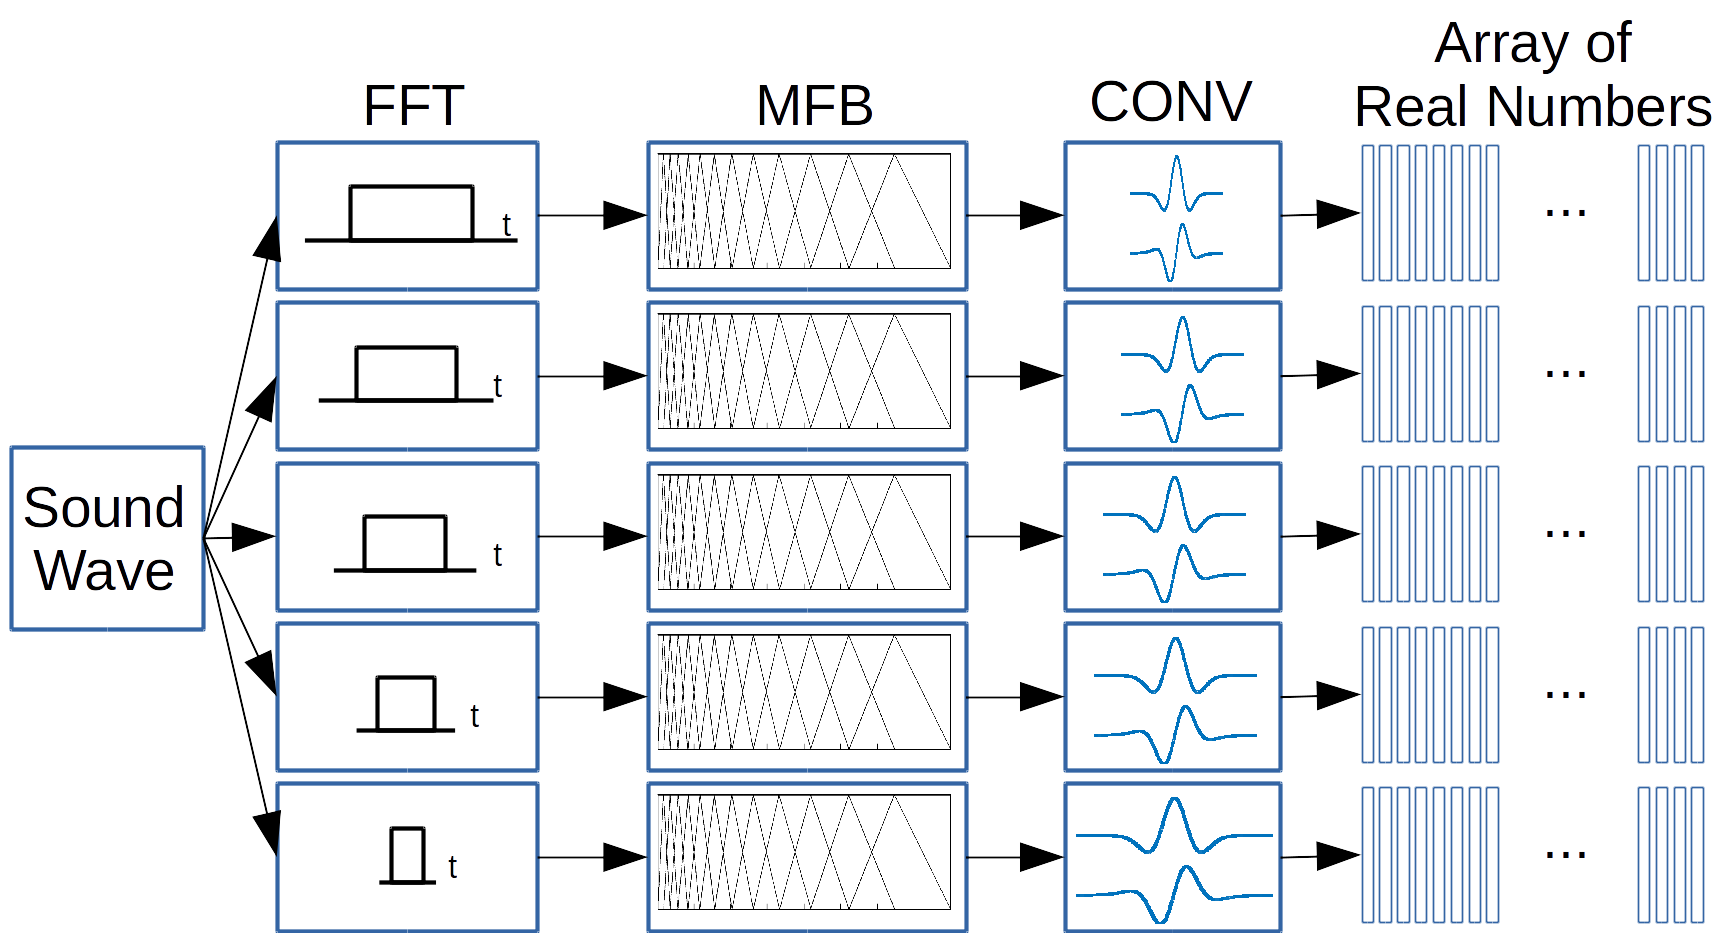
\includegraphics[width=0.8\textwidth]{MRSTSA.png}
    \caption{Algoritmo \glsfirst{mrstsa}. Las ondas de sonido son procesadas por \glspl{fft} con ventanas de tiempo diferentes, luego cada espectro es procesado por
    un \glsfirst{mfb} y cada resolución es convolucionada con una señal compleja con un coeficiente diferente. Luego, el coeficiente de cada filtro
    es obtenido computando el módulo desde la convolución y aplicando control automático de ganancia.}
    %\caption{\glsfirst{mrstsa} algorithm. Sound waves are processed by \glspl{fft} with different time windows, then each spectrum is processed by
    %a \glsfirst{mfb} and each resolution is convolved with a complex signal with a different coefficient. Then, each filter coefficient
    %is obtained computing the modulus from the convolution and then applying a authomatic gain control.}
    \label{fig:MRSTSA}
\end{figure}

Luego, convolucionamos cada resolución obtenida en el último paso a lo largo de su eje tonotópico con una función multiresolución compleja cuya parte real es un sobrero Mexicano simétrico y su parte imaginaria es su transformada antisimétrica de Hilbert. Los coeficientes de la función son 10 para la ventana de tiempo de 8 ms, 8 para la ventana de tiempo de 16 ms, 6 para la ventana de tiempo de 32 ms, 4 para la ventana de tiempo de 64 ms y 2 para la ventana de tiempo de 128 ms (Fig.\ref{fig:MRSTSA}). Con esta estrategia incorporamos el fenómeno de simetría \cite{shamma_1993}, ancho de banda \cite{schreiner_1990} y selectividad a la modulación de frecuencia \cite{shamma_1993,heil_1992,mendelson_1985} hallada en \gls{a1} e incorporado en el algoritmo original \cite{wang_1995}.

%Then, we convolved each resolution obtained in the last step along its tonotopic axis with a complex multiresolution function whose real part was a symmetric Mexican hat function and its imaginary part was its antisymmetric Hilbert transform. The function coefficients are 10 for the 8 ms time window, 8 for the 16 ms time window, 6 for the 32 ms time window, 4 for the 64 ms time window and 2 for the 128 ms time window (Fig.\ref{fig:MRSTSA}). With this strategy we incorporated the phenomena of symmetry \cite{shamma_1993}, bandwidth \cite{schreiner_1990} and frequency modulation selectivity \cite{shamma_1993,heil_1992,mendelson_1985} found in \gls{a1} and incorporated in the original algorithms \cite{wang_1995}.

Obtuvimos la magnitud de cada convolución y aplicamos normalización a cada ventana de tiempo como un control automático de ganancia para priorizar la información entregada por la configuración espectral y no por los valores absolutos entregados por los filtros. Por medio de este mecanismo estamos teniendo en cuenta las propiedades químicas y mecánicas de las células poliosas en el oído interno de los mamíferos las cuales constituyen un mecanismo de transducción el cual parece adaptarse a la historia reciente en los estímulos de manera que puede afectar su ganancia \cite{eatock_2000,holt_2000,le_goff_2005}. Decidimos ser conservativos y no incluir la dimensión de intensidad de sonido sólo incluyendo la silueta en las respuestas de los filtros. 

%We obtained the magnitude of each convolution and applied normalization to each time window as a mean of automatic gain control in order to prioritize the information delivered by the spectral configuration and not the absolute values delivered by the filters. By means of this constraint we account for the mechanical and chemical properties of hair cells in the mammalian inner ear which constitute a transduction mechanism that appears to adapt to recent stimulus history in a way that can affect its gain \cite{eatock_2000,holt_2000,le_goff_2005}. We decided to be conservative, not including sound intensity dimension but just the shape of the filter responses.

Por medio de este procedimiento desde el archivo de audio obtuvimos una respuesta multiresolución espectro-temporal compuesta por un arreglo de 128 columnas--una columna por filtro--y 5 filas--una fila por resolución--con números reales cuyo rango se encuentra entre 0 y 1, para cada paso de tiempo.

%By this procedure we obtained from the audio file a multiresolution spectro-temporal response composed by an array of 128 columns--one column per filter--and 5 rows--one row per resolution--with real numbers which range from 0 to 1, for each time step.




\section{Implementación}

\subsection{Análisis Multiresolución Espectro-Temporal de Sonidos (AMRETS)}

Aplicamos la \gls{fft} a los archivos de audio con un período de muestreo de 8 milisegundos.
A tales efectos utilizamos le paquete FFTW \cite{FFTW05, fftw} con ventanas de tiempo de 8, 16, 32, 64 y 128 milisegundos a los fines de obtener un análisis espectral de potensia de miltiple resolución de la señal.
Adicionalmente, aplicamos la técnica de Banco de Filtros Mel con 128 filtros para cada resolución espectral y convolucionamos tales filtros a lo largo de su ejes tonotópicos. Para la convolución utilizamos una función compleja de resolución múltiple cuya parte real is una función de Sombrero Mexicano y su parte imaginaria es su transformación de Hilbert.

Los valores de los coeficientes de la función son 10 para un tiempo de ventana de 8 milisegundos, 8 para un tiempo de ventana de 16 ms, 6 para un tiempo de ventana de 32 milisegundos, 4 para un tiempo de ventana de 64 milisegundos y 2 para un tiempo de ventana de 128 milisegundos.
Luego computamos la magnitud de la convolución y normalizamos en cada paso temporal.
Por medio de este procedimiento obtenemos desde el archivo de audio una respuesta espectro-temporal de multiple resolución compuesta por un arreglo de 128 columnas--una columna por filtro--y 5 filas--una fila por resolución--de npumeros reales con un rango de 0 a 1 fara cada paso temporal.


%We apply \gls{fft} to the audio files with a sample period of 8 milliseconds.
%We use the FFTW package \cite{FFTW05, fftw}
%with time windows of 8, 16, 32, 64 and 128 milliseconds in order to obtain
%a multiresolution power spectral analysis of the signal.
%%We then applied 
%In addition, we apply the Mel Filter-Bank technique with 128 filters to each
%spectral resolution and convolve such filters along their tonotopic axis.
%For the convolution, we use a multiresolution complex function whose real part
%is a Mexican hat function and its imaginary part is the corresponding Mexican hat Hilbert transformation.
%%-Fig. \ref{fig:Multi}.

%%\begin{figure}[h!]
    %%\centering
    %%\includegraphics[width=0.7\textwidth]{Multi.png}
    %%\caption{Multiresolution complex kernels. Such kernels are convolved with Mel Filter Bank outputs along their tonotopic axis.
	    %%Each kernel has a different coefficient
    %%and is convolved with its corresponding power spectral resolution.
    %%The function coefficients are 10 for 8 ms time window, 8 for 16 ms time window, 6 for 32 ms time window, 4 for 64 ms time window
    %%and 2 for 128 ms time window.}
    %%\label{fig:Multi}
%%\end{figure}

%The function coefficients are 10 for the 8 ms time window, 8 for the 16 ms time window, 6 for the 32 ms time window, 4 for the 64 ms time window
%and 2 for the 128 ms time window. We then compute the magnitude from the convolution and normalize in each time step.
%By means of this procedure we obtain from the audio file a multiresolution spectro-temporal response composed by
%an array of 128 columns--one column per filter--and 5 rows--one row per resolution--with real numbers which range from
%0 to 1, for each time step.



\subsection{Encoder Layer (EL)}

Implementamos un \gls{el} con 225 \glspl{csom} organizados en un arraglo de dos dimensiones de 15 por 15 \glspl{cc}.
Cada \gls{cc} es automáticamente distribuida utilizando ubicaciones individuales a lo largo de sus entradas aferentes de manera uniforme.
Cada \gls{cc} recibe información aferente a través de campos receptivos aferentes bi-dimensionales de 5 por 227 filtros centrados en posiciones individuales sobre el \gls{mrstsa}.
Abilitamos la propiedad de envoltura (wraparound) para lograr que cada campo receptivo ocupe el arreglo del \gls{mrstsa} por completo.
También instruimos a cada columna para que reciba solo 31 entradas, lo cual constituye un porcentaje menor del campo receptivo.
Las entradas aferentes individuales para cada \gls{cc} son escojidas aleatoriamente durante el proceso de inicialización del \gls{el}.

Para esta instancia del modelo, implementamos solo ramificaciones dendríticas laterales ya que no existe más \glspl{cl} de donde traer información por medio de ramificaciones dendríticas apicales.
Configuramos cada \gls{cc} para que tenga un campo receptivo lateral de 9 por 9 \glspl{cc} vecinas y para recibir información de 72 de las 81 \glspl{cc} in el campo receptivo--un 90\% del campo receptivo.


Cada \gls{cc} está compuesta de un arreglo bi-dimensional con 15 por 15 (225) unidades neuronales y cada unidad en una columna podría ser conectada potencialmente con solo 6 unidades neuronales en cada columna vecina vinculada.
De esta manera, cada unidad neuronal en una \gls{cc} termina teniendo 72 ramificaciones dendríticas con 6 conecciones potenciales cada una (432 sinapsis potenciales distantes por unidad celular).
Tales conecciones potenciales se seleccionan de manera aleatoria para cada unidad celulary para cada rama dendrítica en la célula durante el proceso de inicialización del Encoder. El \gls{el} consiste de 50625 unidades celulares con 1569375 sinapsis potenciales y 21870000 sinapsis distantes.
Tales especificaciones determinan el npumero de parámetros libres del modelo, sin embargo, es importante resaltar que las sinapsis distantes representan conecxiones potenciales desde las que solo un pequeño porcentaje tiene un peso sináptico significativo como para ser consideradas conexiones establecidas.
Las sinapsis débiles son periódicamente descartadas por medio de procesos homeostáticos in la red dejando las dendritas distantes con una conectividad dispersa en los campos receptivos. Dispersiones típicas in tales conectividades podrían exeder el 90\%.

Entrenamos el \gls{el} utilizando corpus de 500 palabras generados por el procedimiento descripto en la sección \nameref{CorpGen}.
El procedimiento de entrenamiento consiste de 4 stapas y para cada etapa el \gls{el} recibe el mismo corpus 4 veces.

Durante cada etapa de aprendizaje, ciertos parámetros--como las tasas de aprendizaje en sinapsis próximas y distantes y la iteracción intracolumnar lateral--son decrementadas progresivamente exponencialmente desde un valor inicial, el cual también es decrementado en cada etapa sucesiva.
Una etapa adicional es ejecutada con los parámetros de aprendizaje fijos.

La dispersión en la activación para cada \gls{cc} es 99\% (solo 2 unidades neuronales de las 225 podrían ser activadas por medio de eventos normales de activación).
Por otro lado, la exitación aferente afecta el 10\% de las unidades dentro de los cúmulos en cada \gls{cc}
(22 unidades neuronales, las cuales podrían ser activadas en caso de un \gls{mfe}; Fig. \ref{fig:Activation}).

Cada \gls{cc} esta compuesta de un arreglo bi-dimensional con 15 por 15 (225) unidades neuronales y
cada unidad en una columna podría ser connectada potencialmente con sólo 6 unidades neuronales desde cada columna vecina vinculada.
(432 sinapsis distales por unidad celular).


%We implement an \gls{el} with 225 \glspl{csom} arranged in a two-dimensional
%array of 15 by 15 \glspl{cc}. Each \gls{cc} is automatically distributed using individual locations along its afferent inputs in a uniform way.
%Each \gls{cc} receives afferent information by means of
%two-dimensional afferent receptive fields of 5 by 227 filters centered at individual locations over the \gls{mrstsa}.
%We enable the wraparound property in order to make each receptive field span the entire
%\gls{mrstsa} array.
%We also instruct each column to receive only 31 inputs, which is a minor percentage of such
%receptive field.
%Individual afferent inputs for each \gls{cc} are chosen randomly in the \gls{el} initialization. 

%For this model instance we implement only distal lateral dendritic branches since there are
%no more \glspl{cl} from which to bring information through apical dendritic branches.
%We configure each \gls{cc} to have a lateral receptive field with 9 by 9 neighboring \glspl{cc}
%and to receive information from 72 of the 81 \glspl{cc} in the receptive field--a 90\% of the receptive field.

%Each \gls{cc} is composed of a two-dimensional array with 15 by 15 (225) neural units and
%each unit in a column could be potentially connected with only 6 neural units from each linked neighboring column. 
%That is, each neural unit in a \gls{cc} ends up with 72 lateral dendritic branches with 6 potential connections each
%(432 distal potential synapses per cellular unit).
%Such potential synapses are randomly chosen for each neural cell and for each dendritic branch in the cell during the Encoder initialization procedure.
%The \gls{el} consists of 50625 cellular units with 1569375 proximal synapses and 21870000 distal synapses.
%\reviewerfour{Such specifications state the number of free parameters of the model, but it is important to highlight that distal synapses represent
%potential connections from which only a small percentage has a significant synaptic weight as to be considered as an established connection.
%Weak synapses are periodically pruned by means of homeostatic processes in the network leaving distal dendrites with a sparse connectivity in the receptive fields.
%Typical sparseness in such connectivity matrices could exceed the 90\%.}

%We train the \gls{el} using a 500 word corpora generated by the procedure described in section \nameref{CorpGen}.
%The training procedure consists of 4 stages and for each stage the \gls{el} receives the same corpus 4 times.

%During each learning stage, certain parameters--such as the learning rates in proximal and distal synapses and the lateral
%intra-column interaction--are exponentially and progressively decreased from an initial value, which also decreases
%for each successive stage.
%An additional stage is executed with the learning parameters fixed.

%The sparsity in the activation for each \gls{cc} is 99\% (just 2 neural units out of 225 could be active for normal activation events).
%On the other hand, the afferent excitation affects 10\% of the units inside the clusters in each \gls{cc}
%(22 neural units, which could be activated in case of a \gls{mfe}; Fig. \ref{fig:Activation}).








\subsection{Clasificación por medio de Support Vector Machine (SVM)}

Utilizamos supervisión con clasificación por medio del método \gls{svm}, recibiendo las salidas de cada algoritmo \cite{CC01a, libsvm}. Hacemos eso para probar las propiedades de invarianza en las características fonéticas abstraidas por el \gls{el} en comparación con las propiedades fonéticas abstraidas por el \gls{mrstsa}, 
(Fig. \ref{fig:Experiment}).

Utilizamos las brechas temporales de silencio entre palabras consecutivas en las salidas del \gls{mrstsa} para introducir marcas y así detectar el pricipio y el final de cada palabra.

Luego, producimos un vector por palabra en el corpus sumando la actividad en el \gls{mrstsa} así como en el \gls{el} entre marcas consecutivas
y utilizamos tales vectoresjpara entrenar ambos clasificadores (el que recibe las salidas provenientes desde el \gls{mrstsa} y el que las recibe desde el \gls{el}).

Luego, escalamos los vectores--como la documentación del \gls{libsvm} sugiere--para mejorar el desempeño en la clasificación.
Entrenamos y probamos los clasificadores \gls{svm} utilizando validación cruzada sobre 5 secciones y los configuramos para utilizar un kernel linear con un parámetro $C$ el cual barremos para encontrar el mejor modelo entrenado para cada clasificador.



%We use supervision by means of the \gls{svm} classification
%method, receiving the outputs from each algorithm \cite{CC01a, libsvm}. We do this to test the invariance properties in the phonetic features abstracted by the \gls{el} in comparison
%with the phonetic features abstracted by the \gls{mrstsa}, 
%(Fig. \ref{fig:Experiment}).

%We use the silent temporal gaps between consecutive words in the \gls{mrstsa} outputs in order to introduce marks to
%detect the beginning and end of each word.

%We then produce a vector per word in the corpus summing the activity in the \gls{mrstsa} as well as in the \gls{el} between consecutive marks
%and use such vectors to train both classifiers (the one receiving outputs from the \gls{mrstsa} and the one receiving outputs from the \gls{el}).

%Afterwards, we scale the vectors--as the \gls{libsvm} documentation suggests--
%so as to improve the classification performance.
%We train and test the \gls{svm} classifiers using 5-fold cross-validation
%and configure them to use a linear kernel with one parameter $C$ which
%we swept to find the best trained model for each classifier.


\section{Experimentos}

\section{Resultados}

\section{Discusión}

\section{Conclusiones}
